\section{Vektorrechner}

\begin{defi}[Vektorprozessoren]{Idee}
    Mathematisch-technische Anwendungen lassen sich erheblich in der Ausführung beschleunigen,
    wenn für Vektoroperationen:
    \begin{itemize}
        \item Spezielle, schnelle Hardware zur Verfügung steht und
        \item in der Programmiersprache Konstrukte zur Beschreibung von Vektor-Operationen verhanden sind
              (HPC Fortran, und zum Teil auch Fortran 90) oder
        \item der Compiler automatisch Programmteile als vektorisierbar erkennt
              (zum Teil mit Hilfe von Direktiven)
    \end{itemize}
    Mögliche Operationen (meist beschränkt auf Floating Point):
    \begin{itemize}
        \item $v = v \pm v, v = s \pm v$
        \item $v = v \cdot v, v = s \cdot v$
        \item mit n-elementigem Vektor $v$ und Skalar $s$
    \end{itemize}
    Eine Division wurde zunächst mit Hilfe einer Reziprok-Funktionseinheit berechnet:
    $v = \frac{1.0}{v}$
\end{defi}

\begin{defi}[Vektorprozessoren]{Ziel}
    Mit (im Idealfall!) einer Vektoroperation können gleichzeitig alle Elemente von zwei Vektoren verknüpft werden:
    \begin{align*}
        vc[1] & = va[1] \pm vb[1] \\
        \vdots                    \\
        vc[n] & = va[n] \pm vb[n]
    \end{align*}
    Dies braucht (im Idealfall!) für alle $n$ Elemente nicht mehr Rechenzyklen als die Berechnung für eine entsprechende Skalaroperation.
    Analog zum \enquote{Instruction Level Parallelism}[TODO: ref] (ILP) ist das Vector Processing eine Form des \enquote{Data Level Parallelism} (DLP).
\end{defi}

\begin{defi}{Data Level Parallelism (DLP)}
    \emph{Data Level Parallelism (DLP)} oder Datenparallelität ist die Parallelisierung über mehrere Prozessoren in parallelen Rechenumgebungen.
    Sie konzentriert sich auf die Verteilung der Daten auf verschiedene Knoten, die die Daten parallel bearbeiten.
    Sie kann auf reguläre Datenstrukturen wie Arrays und Matrizen angewendet werden, indem jedes Element parallel bearbeitet wird.
\end{defi}

\begin{defi}{Vektor-Pipeline}
    TODO: Sinnvolle Definition
\end{defi}

\begin{defi}{Aufbau CPU vs. GPU}
    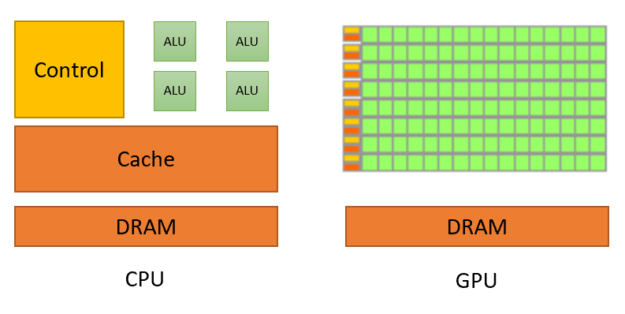
\includegraphics[width=\textwidth]{images/CPUvsGPU.png}
    % TODO: Pradeep Gupta, CUDA Refresher: Reviewing the Origins of GPU Computing, \url{CUDA Refresher: Reviewing the Origins of GPU Computing}, zuletzt aufgerufen am 17.06.2023

    Mit \enquote{ALU} als \enquote{algorithmic logic unit} oder \enquote{arithmetisch-logische Einheit}.

    Die CPU verfolgt das Konzept der geringen Latenz,
    wobei die GPU eine hohe Bandbreite anstrebt.
\end{defi}

\begin{defi}{GPU}{Programmausführung}
    \begin{enumerate}
        \item Kopieren der Eingabedaten vom CPU Speicher in den DRAM der GPU.
        \item Laden und Ausführen des Programms auf der GPU,
              wobei Caching für eine bessere Performance genutzt wird.
        \item Kopieren der Ergebnisse vom DRAM der GPU zurück in den CPU Speicher.
    \end{enumerate}
\end{defi}

\begin{defi}{Field Programmable Gate Array (FPGA)}
    \begin{itemize}
        \item Integrierter Schaltkreis, der vom Anwender selbst (anwendungsspezifisch) konfiguriert werden kann.
        \item Enthält eine Vielzahl von Logikschaltungen wie AND, XOR (bis zu mehreren Millionen Gatter).
        \item Einzelne Komponenten können hierarchisch und beliebig miteinander verschaltet werden.
        \item Logikblöcke enthalten in der Regel Speicher-Blöcke (z.B. Flip-Flops).
        \item Können je nach Bauart mehrfach oder nur einmal programmiert werden (Schmelzbrücken).
    \end{itemize}
\end{defi}

\begin{defi}[Field Programmable Gate Array (FPGA)]{Anwendungen}
    \begin{itemize}
        \item Es existiert eine Hardware Description Language (HDL) zur Konfiguration eines FPGAs, wobei Tools wie z. B. HDL Coder von MathWorks verfügbar sind.
        \item Ermöglichen effizientes Lösen komplexer und sehr spezifischer Aufgaben.
        \item Können genutzt werden, um Chip-Design (ASIC) und Funktionalität vorab zu testen, bevor die implementierte Logik als Chip produziert wird.
        \item Eignen sich ebenfalls als Beschleuniger, z.B. in Kombination mit einer Host-CPU.
        \item Schnelle Anbindung über QPI (QuickPath Interconnect, Intel) oder über PCIe.
    \end{itemize}
\end{defi}

\subsection{Aufgaben}

\begin{aufgabe}{Vektorprozessoren}
    Welche Eigenschaften müssen die Programmiersprache bzw. der Compiler haben um Vektorprozessoren nutzen zu können?
    \tcblower
    Die Programmiersprache muss Konstrukte zur Beschreibung der Vektoroperationen enthalten
    \underline{oder} der Compiler muss automatisch Programmteile als vektorisierbar erkennen.
\end{aufgabe}

\begin{aufgabe}{Parallelität}
    Erklären Sie den Unterschied zwischen ILP und DLP.
    \tcblower
    \begin{itemize}
        \item \emph{ILP (Instruction-Level Parallelism)} bezieht sich auf die Fähigkeit eines Prozessors,
              mehrere Anweisungen gleichzeitig auszuführen,
              indem er Anweisungen analysiert und versucht,
              Anweisungen zu finden,
              die unabhängig voneinander ausgeführt werden können.
              Der Prozessor kann dann diese Anweisungen parallel ausführen,
              um die Geschwindigkeit der Ausführung zu erhöhen.
        \item \emph{DLP (Data-Level Parallelism)} hingegen bezieht sich auf die Fähigkeit eines Prozessors,
              mehrere Datenströme parallel zu verarbeiten.
              Ein Beispiel für DLP ist die Verwendung von Vektorprozessoren,
              die in der Lage sind,
              mehrere Elemente eines Vektors gleichzeitig zu verarbeiten.
    \end{itemize}
\end{aufgabe}

\begin{aufgabe}{Vektorpipeline}
    Durch welche 3 Architekturkonzepte lässt sich die Datenverarbeitung mittels Vektorpipeline beschleunigen ?
    \tcblower
    \begin{itemize}
        \item Vektor-Pipleline Chaining
        \item Load/Store parallel zur Data Pipeline
        \item Load/Store Chaining
    \end{itemize}
\end{aufgabe}

\begin{aufgabe}[Pipelining]{ILP}
    Bei RISC-Prozessoren mit Pipelining ist eine Überlappung der Befehle bei der Ausführung möglich.
    Welcher Effekt kann diese Überlappung verhindern?
    \tcblower
    Register-Naming-Hazard
\end{aufgabe}

\begin{aufgabe}[Vektorpipeline]{Memory-Zugriffe}
    Welcher Effekt tritt beim unmittelbar nacheinander erfolgenden Zugriff auf Speicheradressen derselben Memory-Bank auf?
    \tcblower
    Totzeit des Speichers
\end{aufgabe}

\begin{aufgabe}[Vektorpipeline]{Memory-Zugriffe}
    Durch welche zwei Varianten kann ein Stride beim Zugriff auf die Memory-Bänke erzeugt werden?
    \tcblower
    \begin{itemize}
        \item explizit, d.h. durch Angabe der Schrittweite beim Schleifendurchlauf
        \item implizit durch Anordnung der Array-Elemente im Memory,
              sowie die Reihenfolge des Zugriffs auf diese
    \end{itemize}
\end{aufgabe}

\begin{aufgabe}{MSA}
    Beschreiben Sie kurz den Vorteil der MSA im Hinblick auf Beschaffungskosten von Superrechnern.
    \tcblower
    \begin{itemize}
        \item Es können einzelne Module ersetzt und mit bestehender HW verknüpft werden,
              das heißt,
              es muss nicht der komplette Supercomputer erneuert werden
        \item einzelne Module können unterschiedliche finanziert werden,
              z.B. durch verschiedene Fördertöpfe (Bund, Land)
    \end{itemize}
\end{aufgabe}